\documentclass[12pt]{article}
\usepackage{proposal}
\usepackage{listofauthorships}
\usepackage{multicol}

\title{\scshape MQP Project Proposal}
\author{Samuel Goldman, Evan Goldstein, Christopher Myers, David Vollum}
% \date{September 2019}

\makeglossaries
% \todo{Fix numbering}
% Acronyms
% Follow the form: \newacronym{label}{ACRONYM}{expansion}
% Also: alphabetize!
\newacronym{api}{API}{application programming interface}
\newacronym{aws}{AWS}{Amazon Web Services}
\newacronym{caida}{CAIDA}{Center for Applied Internet Data Analysis}
\newacronym{cdf}{CDF}{cumulative distribution function}
\newacronym{cli}{CLI}{command-line interface}
\newacronym{cors}{CORS}{cross-origin resource sharing}
\newacronym{csv}{CSV}{comma separated value}
\newacronym{ddos}{DDoS}{distributed denial of service}
\newacronym{dns}{DNS}{domain name system}
\newacronym{dsl}{DSL}{digital subscriber line}
\newacronym{fcc}{FCC}{Federal Communications Commission}
\newacronym{gdp}{GDP}{gross domestic product}
\newacronym{gis}{GIS}{geographic information system}
\newacronym{gps}{GPS}{global positioning system}
\newacronym{html}{HTML}{Hypertext Markup Language}
\newacronym{http}{HTTP}{hypertext transfer protocol}
\newacronym{httpse}{HTTPS}{hypertext transfer protocol secure}
\newacronym{idw}{IDW}{inverse distance weighting}
\newacronym{iqr}{IQR}{inter-quartile range}
\newacronym{ip}{IP}{internet protocol}
\newacronym{ipaoc}{IPoAC}{internet protocol over avian carrier}
\newacronym{ipvs}{IPv6}{internet protocol version 6}
\newacronym{ipvf}{IPv4}{internet protocol version 4}
\newacronym{json}{JSON}{Javascript Object Notation}
\newacronym{jwt}{JWT}{\json Web Token}
\newacronym{mbps}{Mbps}{megabits per second}
\newacronym{mqp}{MQP}{major qualifying project}
\newacronym{ntp}{NTP}{Network Time Protocol}
\newacronym{ripe}{RIPE}{R\'eseaux IP Europ\'eens}
\newacronym{rtt}{RTT}{round trip time}
\newacronym{sdk}{SDK}{software development kit}
\newacronym{svg}{SVG}{scalable vector graphics}
\newacronym{tcp}{TCP}{transmission control protocol}
\newacronym{tld}{TLD}{top level domain}
\newacronym{tls}{TLS}{transport layer security}
\newacronym{ttl}{TTL}{time-to-live}
\newacronym{acUrl}{URL}{uniform resource locator}
\newacronym{us}{US}{United States}
\newacronym{usps}{USPS}{United States Postal Service}
\newacronym{voip}{VoIP}{voice over internet protocol}
\newacronym{wpi}{WPI}{Worcester Polytechnic Institute}

% Acronyms with definitions
% Follow the form: \newacronym{label}{ACRONYM}{expansion}{description}. Description appears in glossary only.
\newacronym{anova}{ANOVA}{analysis of variance}{Analysis of variance is a class of statistical models and methods for estimation, used to analyze the difference between the means of a sample. Although there are many types, they all fundamentally calculate the probability (a $p$ value) that two population means are equal}

\newacronym{cdn}{CDN}{content delivery network}{A content distribution network, sometimes called a Content Delivery Network, is a network of proxy servers that form a kind of cache used to enhance delivery of content to internet users. Although helpful for internet users, they complicate measurements of connectivity to websites \textit{actually} connecting to the site's servers}
 
\newacronym{cv}{CV}{coefficient of variation}{Coefficients of variation, or relative standard deviations, are defined as the ratio of the absolute value of the mean of a variable divided by its standard deviation: $\frac{\lvert\mu\rvert}{\sigma}$. CVs are dimensionless values that can be judged independent of the original source, making them useful for gauging the spread of any data set. The lower the CV, the lower the spread of the data and the better the quality}
 
\newacronym{ecc}{EC2}{Amazon Elastic Compute Cloud}{EC2 is a service from Amazon Web Services that provides virtual machines in the cloud for general-purpose or task optimized work. EC2 can be configured for different performance and pricing classes, as well as complex auto-scaling schemes or virtual private cloud setups}
 
\newacronym{etl}{ETL}{extract-transform-load}{Extract-transform-load is a generic procedure for extracting data, transforming it into a more useful format, and loading it into a large volume storage system, such as a database. The term closer describes an architecture rather than a specific algorithm}
 
\newacronym{icmp}{ICMP}{internet control message protocol}{Internet Control Message Protocol is a protocol designed for error reporting and other utility purposes across the internet, typically used most by routers and other intermediary devices}

\newacronym{isp}{ISP}{internet service provider}{An internet service provider is typically the "last mile" organization that provides a user with internet access --- otherwise known as a \textit{tier 3} ISP. They are distinct from tier 2 and tier 1 ISPs which are responsible for much of the internet backbone, although ISP corporations may operate on multiple tiers. Common ISPs in the US include AT\&T, Comcast, and Verizon}
 
\newacronym{kde}{KDE}{kernel density estimation}{Kernel density estimation is a technique for estimating the probability density function of a variable. Briefly, KDEs work by processing each measurement of a variable as if it was at the center of some given probability density function, e.g. a gaussian curve. These curves are then summed together to form one curve and normalized so the area underneath the curve is equal to 1. A KDE chart can be read in the same way as a histogram can, but the $y$ axis corresponds to a density instead of an absolute value. The advantage to using a KDE over a histogram is that KDEs are not vulnerable to binning effects (from choosing the wrong bin size) while histograms are}

% Glossary entries -- these should be more detailed.
% Follow the form: \newglossaryentry{LABEL}{name={NAME} description={YOUR TEXT HERE}}
% \newglossaryentry{favicon}{
%     name={favicon},
%     description={Favicons are small identifying images, typically logos or relevant UI elements, that most websites provide for browsers to place on tabs and bookmarks. Favicons are stored as .ico files (icons) and are either 16x16, 32x32, or 48x48. This small size makes them ideal for testing connection \rtt from a browser}
% }

% \newglossaryentry{backbone}{
%     name={internet backbone},
%     description={Internet backbone infrastructure consists of high speed principal data routes and the connected major computer networks and core routers. For any trip of serious distance (likely most connections, unless you happen to have a data center in your backyard), packets will inevitably pass through some element of the internet backbone}
% }

% \newglossaryentry{traceroute}{
%     name={traceroute},
%     description={A traceroute is a technique that shows the full path data takes to get from your computer to a remote server, and how long it takes to get to each server along the way. Traceroutes leverage \icmp and specifically-set \ttl values to inciteintermediate servers to respond with an \icmp packet indicating the data packet's \ttl has expired -- thereby giving away the server's presence along the route}
% }


\begin{document}
% Title page
\pagenumbering{gobble}
\maketitle
\newpage

% Table of contents, list of authorships, list of figures
\pagenumbering{roman}
\tableofcontents\newpage
% \listofauthorships
\listoffigures
\newpage

% Switch to arabic page numbering, start headers, and one half spacing.
\pagenumbering{arabic}
\pagestyle{fancy}
\onehalfspacing

\section{Introduction}
There are many ways to define "Internet connectivity," and for each definition many ways to measure it. For example, you could focus on the user experience aspect of connectivity and place emphasis on measuring what a typical user would actually do, i.e. loading from domains, not \acrshort{ip}s and accepting that \acrfull{cdn}s and load balancing exist. Additionally, \textit{most} users likely use the \textit{top} websites - user experience analysis would account for this.

On the other hand, a network-centric approach could focus on analyzing the backbones and topology of the internet. This data would be of little use to everyday users, but potentially valuable to network researchers and architects looking to improve connectivity across the country.

This document presents various options for both approaches including how data might be collected, processed, and analyzed.

\newpage

\section{Data Sources and Analysis Methods}
\subsection{Favicon Ping}[Samuel G.]
This method involves distributed users loading a web page that itself continually loads favicons from a set of predetermined, popular websites. Favicons are small identifying images that most major websites provide for browsers to place on tabs. By loading these images with a random parameter to circumvent caching, the page can estimate the round trip time required to receive the favicon, analogous to a ping time. The site then reports this ping, along with the client \acrshort{ip} address, to a server.

Websites would likely be selected using a list of the most popular sites in the world and/or the United States, such as \href{www.alexa.com/topsites}{Alexa} or \href{www.similarweb.com/top-websites}{SimilarWeb}. Using such lists would focus this investigation on the websites that most impact usability of an internet connection for most people.

\paragraph{Potential issues}
Attempting to measure timing data from a browser will introduce jitter and uncertainty into the data, and estimated \acrshort{rtt}s will not be representative of a true ping with \acrfull{icmp} packets. Additionally, the analysis might have to account for different browsers impacting load time, although we have not yet explored this.

\subsubsection{Multiple IP RTT}[Samuel G.]
When a user loads the data collection page, a script in the background will continually request favicons from a list of the top websites in the United States and measure the total time to get the image. This method only attempts to circumvent favicon caching (by including a randomized parameter) - it ignores the possibility of \acrshort{cdn}s or any other methods of optimizing delivery speeds. We chose to include cache prevention because normal users don't repeatedly load favicons, however in order to collect enough data to eliminate jitter the favicon must be loaded multiple times for each user. By not accounting for \acrshort{cdn}s, this method enables a limited form of normalization by distance: if a website uses a strong \acrshort{cdn}, it accounts for distance in load times, to a certain degree.

\paragraph{How the data is useful}
This data can show approximately how fast users can static resources from the top websites in the country. We can create maps showing connectivity for each targeted website, which would highlight differences for different websites. For example, users in San Francisco may have higher \acrshort{rtt}s for wpi.edu than users in Boston. Additionally, averaging (perhaps with a weight based on popularity) the data for all websites together could show overall connectivity to the websites based on region. Conversely, for each website, this data can show which regions may need either stronger \acrshort{cdn} support or better network connectivity.

\subsubsection{Single IP RTT}[Samuel G.]
When a website uses a \acrshort{cdn} a client loading the web page on the east coast may end up loading Amazon.com's favicon from a different server than a user on the west coast. To circumvent this, the data collection site would load the favicons from a specific \acrshort{ip} address, bypassing DNS resolution.

\paragraph{How the data is useful}
Most people do not load websites from \acrshort{ip} addresses, so this method would not be representative of the experience for everyday users. However, this method has the potential to show the disparity in \acrshort{cdn}s for different sites.

\subsubsection{Single IP RTT per distance}[Samuel G.]
When using the favicon ping method with a single target \acrshort{ip}, post analysis can estimate the approximate distance between the client and the server that sent the favicon. By dividing the average ping between that client and the server, we can normalize the data for distance.

\paragraph{How the data is useful}
While distance is a major factor in load times and overall user experience, normalizing for distance will highlight areas that have a better connection relative to their distance from content providers. However, this would not be representative of usability: users far from content data centers or \acrshort{cdn}s would still suffer from slow load times even if they have a top tier connection. This analysis could show where efforts could be made to improve connections.

\subsubsection{Multiple IP RTT per rated connection speed}[Samuel G.]
Measured \acrshort{rtt} times to domain names (potentially multi-homed) could be normalized to expected connection speeds (see section below) using the size of the loaded favicon ((favicon size / (average \acrshort{rtt} / 2) / expected connection speed). Using this data, locations could be assigned a "getting-what-you-paid-for" index. A higher value would indicate a better connection relative to the expected connection; a lower value would indicate connections worse than expected.

\subsection{CAIDA, RIPE Atlas, \& Measurement Lab Traceroutes}[Chris M.]

The \acrfull{caida}, \acrfull{ripe} Atlas, and Measurement Lab own nodes across the world that routinely run traceroutes to different locations. 

\acrshort{caida} maintains what they call the Archipelago network (or just Arc), a series \textapprox{}180 of Raspberry Pi's across the world that run measurements to different parts of the internet. We're interested in their prefix probing data set, which involves running complete traceroutes to at least one host in every /24 prefix. That is, every day, every Arc node runs a traceroute that picks up on one host in 130.215.1.x address, one in 130.215.2.x, and so on. This produces an \textit{enormous} amount of data, dating back to 2014 with over 6,000 compressed binary files. We have a series of python scripts that can extract this data and shove it into either hundreds of SQLite databases, or one big PostgreSQL database for easier analysis.

\acrshort{ripe} Atlas and Measurement Lab run on approximately the same principle, collecting tens of thousands of traceroutes per day.

To gain a better understanding of the data from \acrshort{caida} we conducted some basic statistic analyses to gauge the spread of the data. The charts below were created using about a sixth of the data available, with only source to final destination routes considered -- effectively just a ping.

\begin{figure}[H]
    \centering
    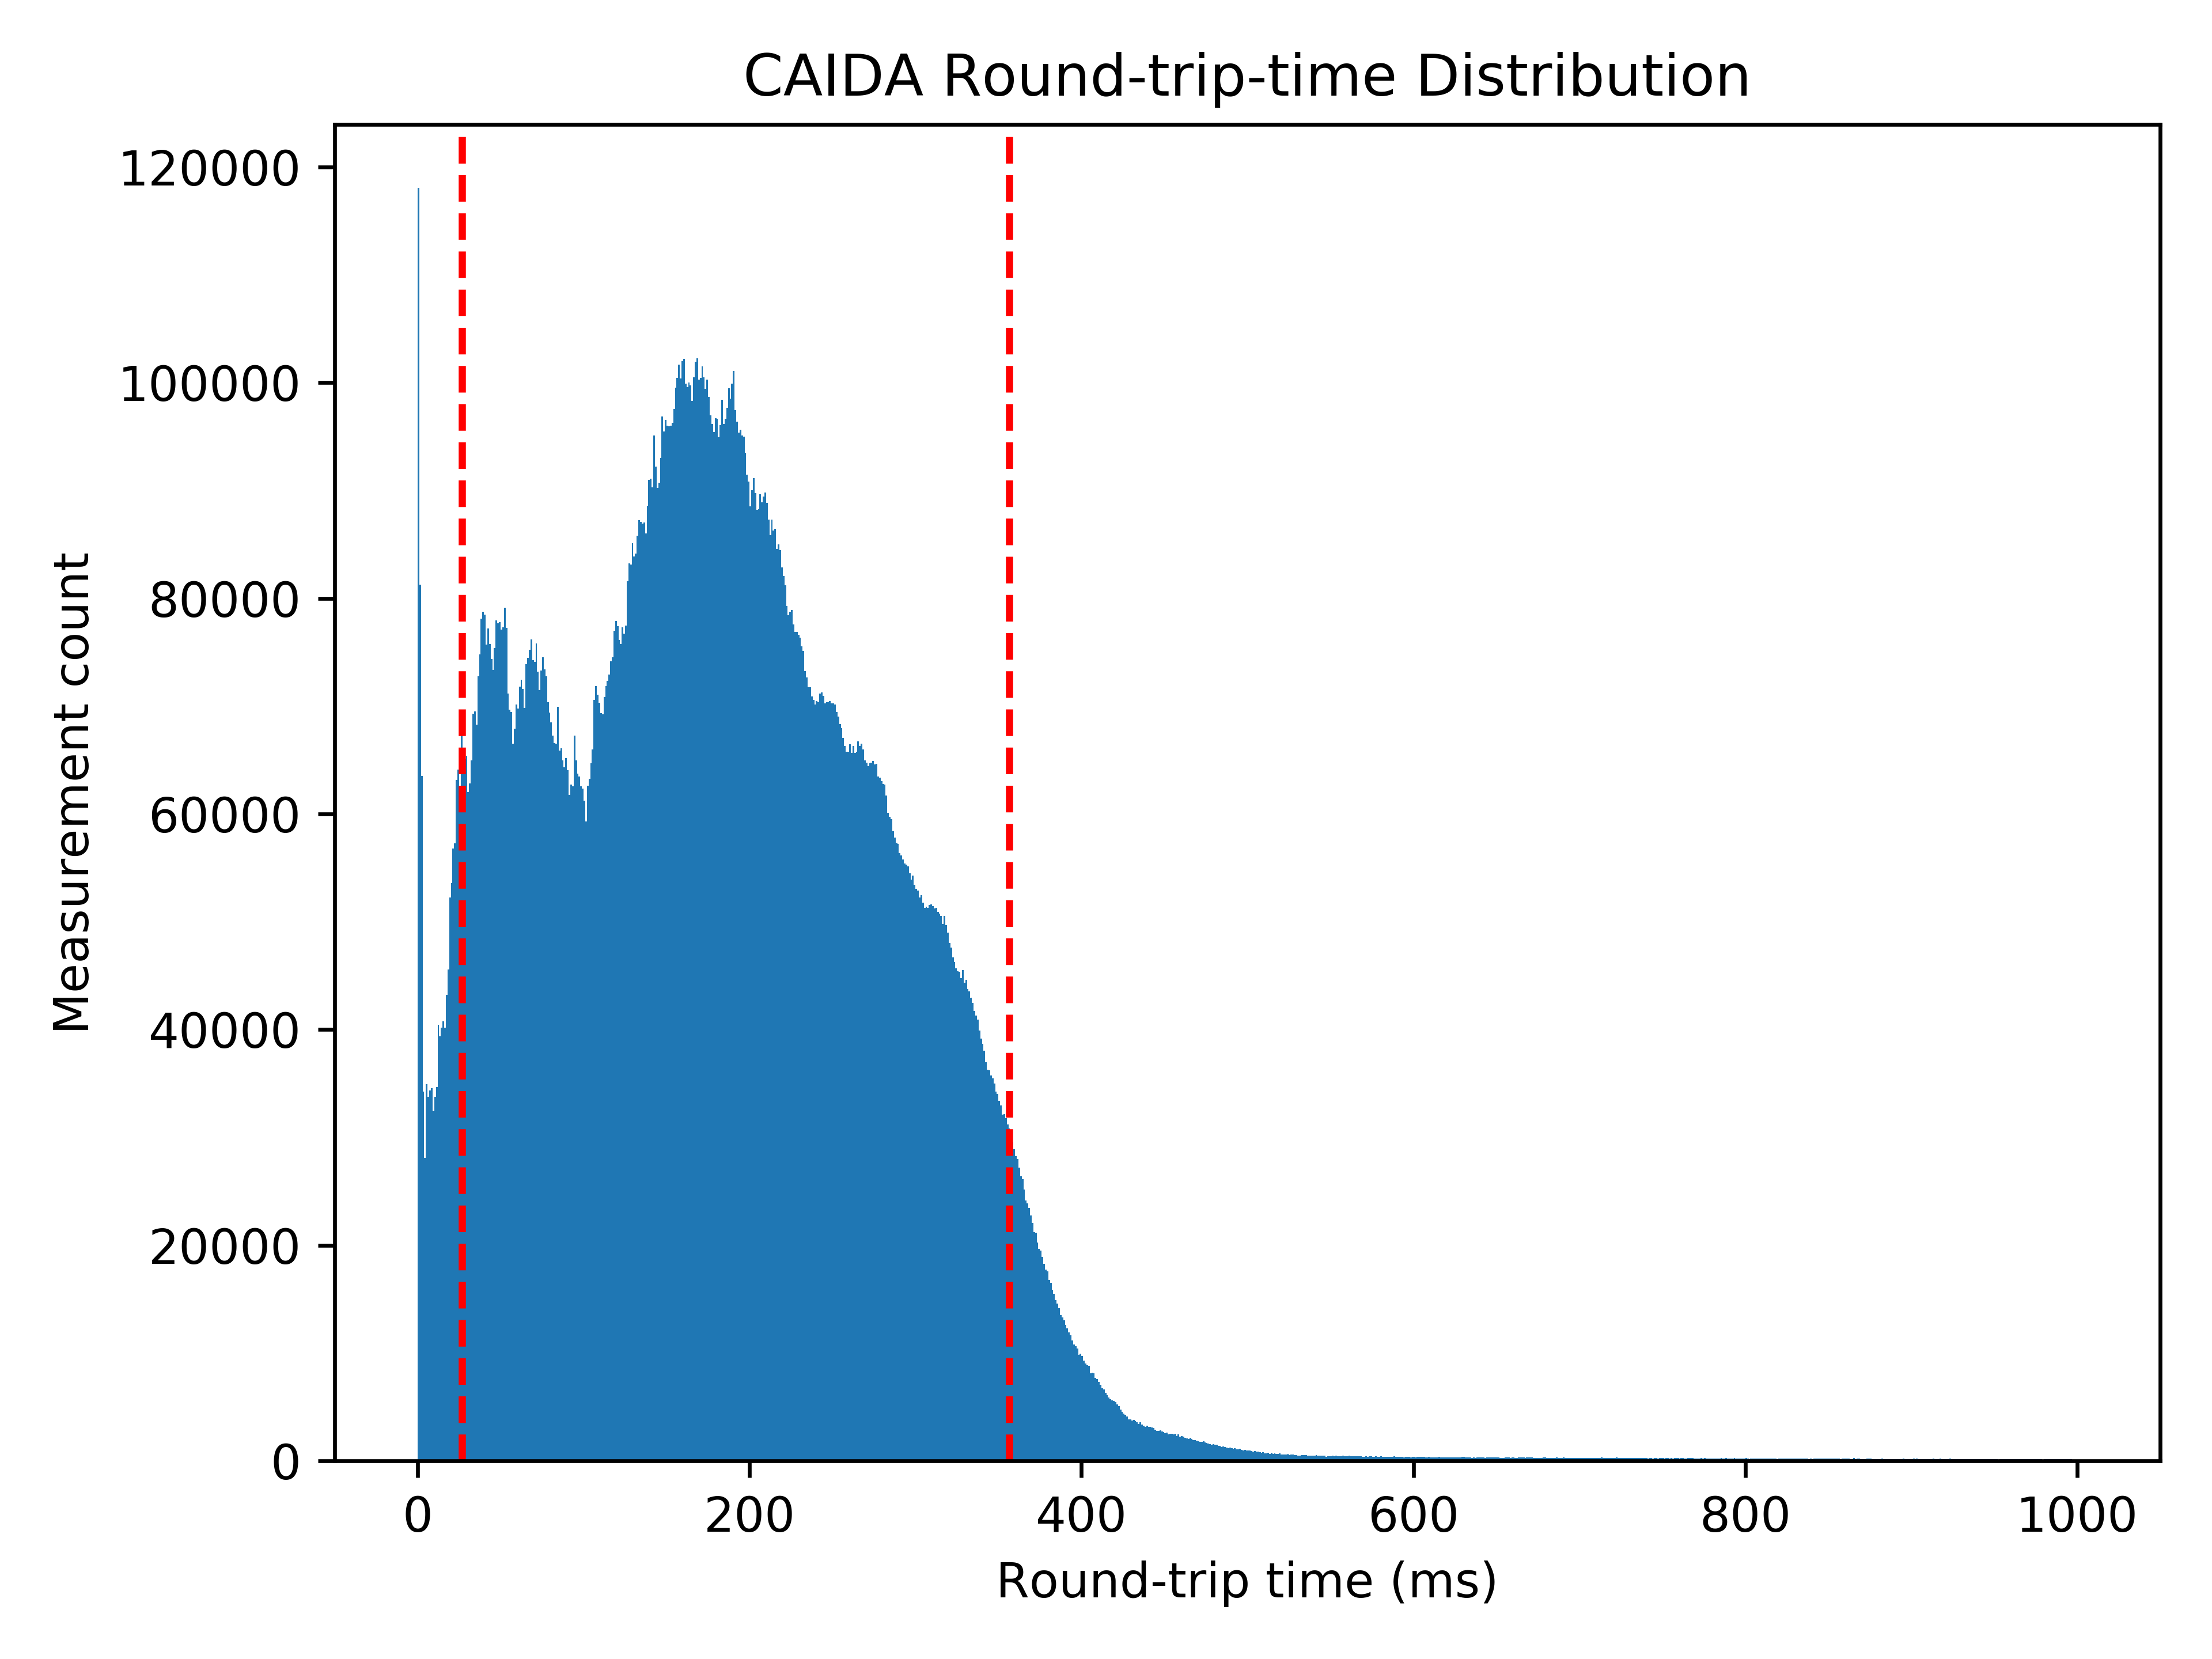
\includegraphics[width=\textwidth]{images/CAIDA_rtt_dist.png}
    \caption{Distribution of CAIDA RTTs with 5th and 95th percentiles shown}
    \label{fig:rtt_dist}
\end{figure}

Figure \ref{fig:rtt_dist} shows the distribution of \acrshort{rtt}s recorded by CAIDA, with extreme values above 1000 ms omitted. The graph shows a reasonably sharp peak with a curious bimodal distribution. Fortunately, this easily explainable -- the two peaks likely represent sources from different landmasses. For instance, the larger peak on the right might correspond to hosts in Europe and Asia, while the smaller peak on the left might correspond to North and South America.

\begin{figure}[H]
    \centering
    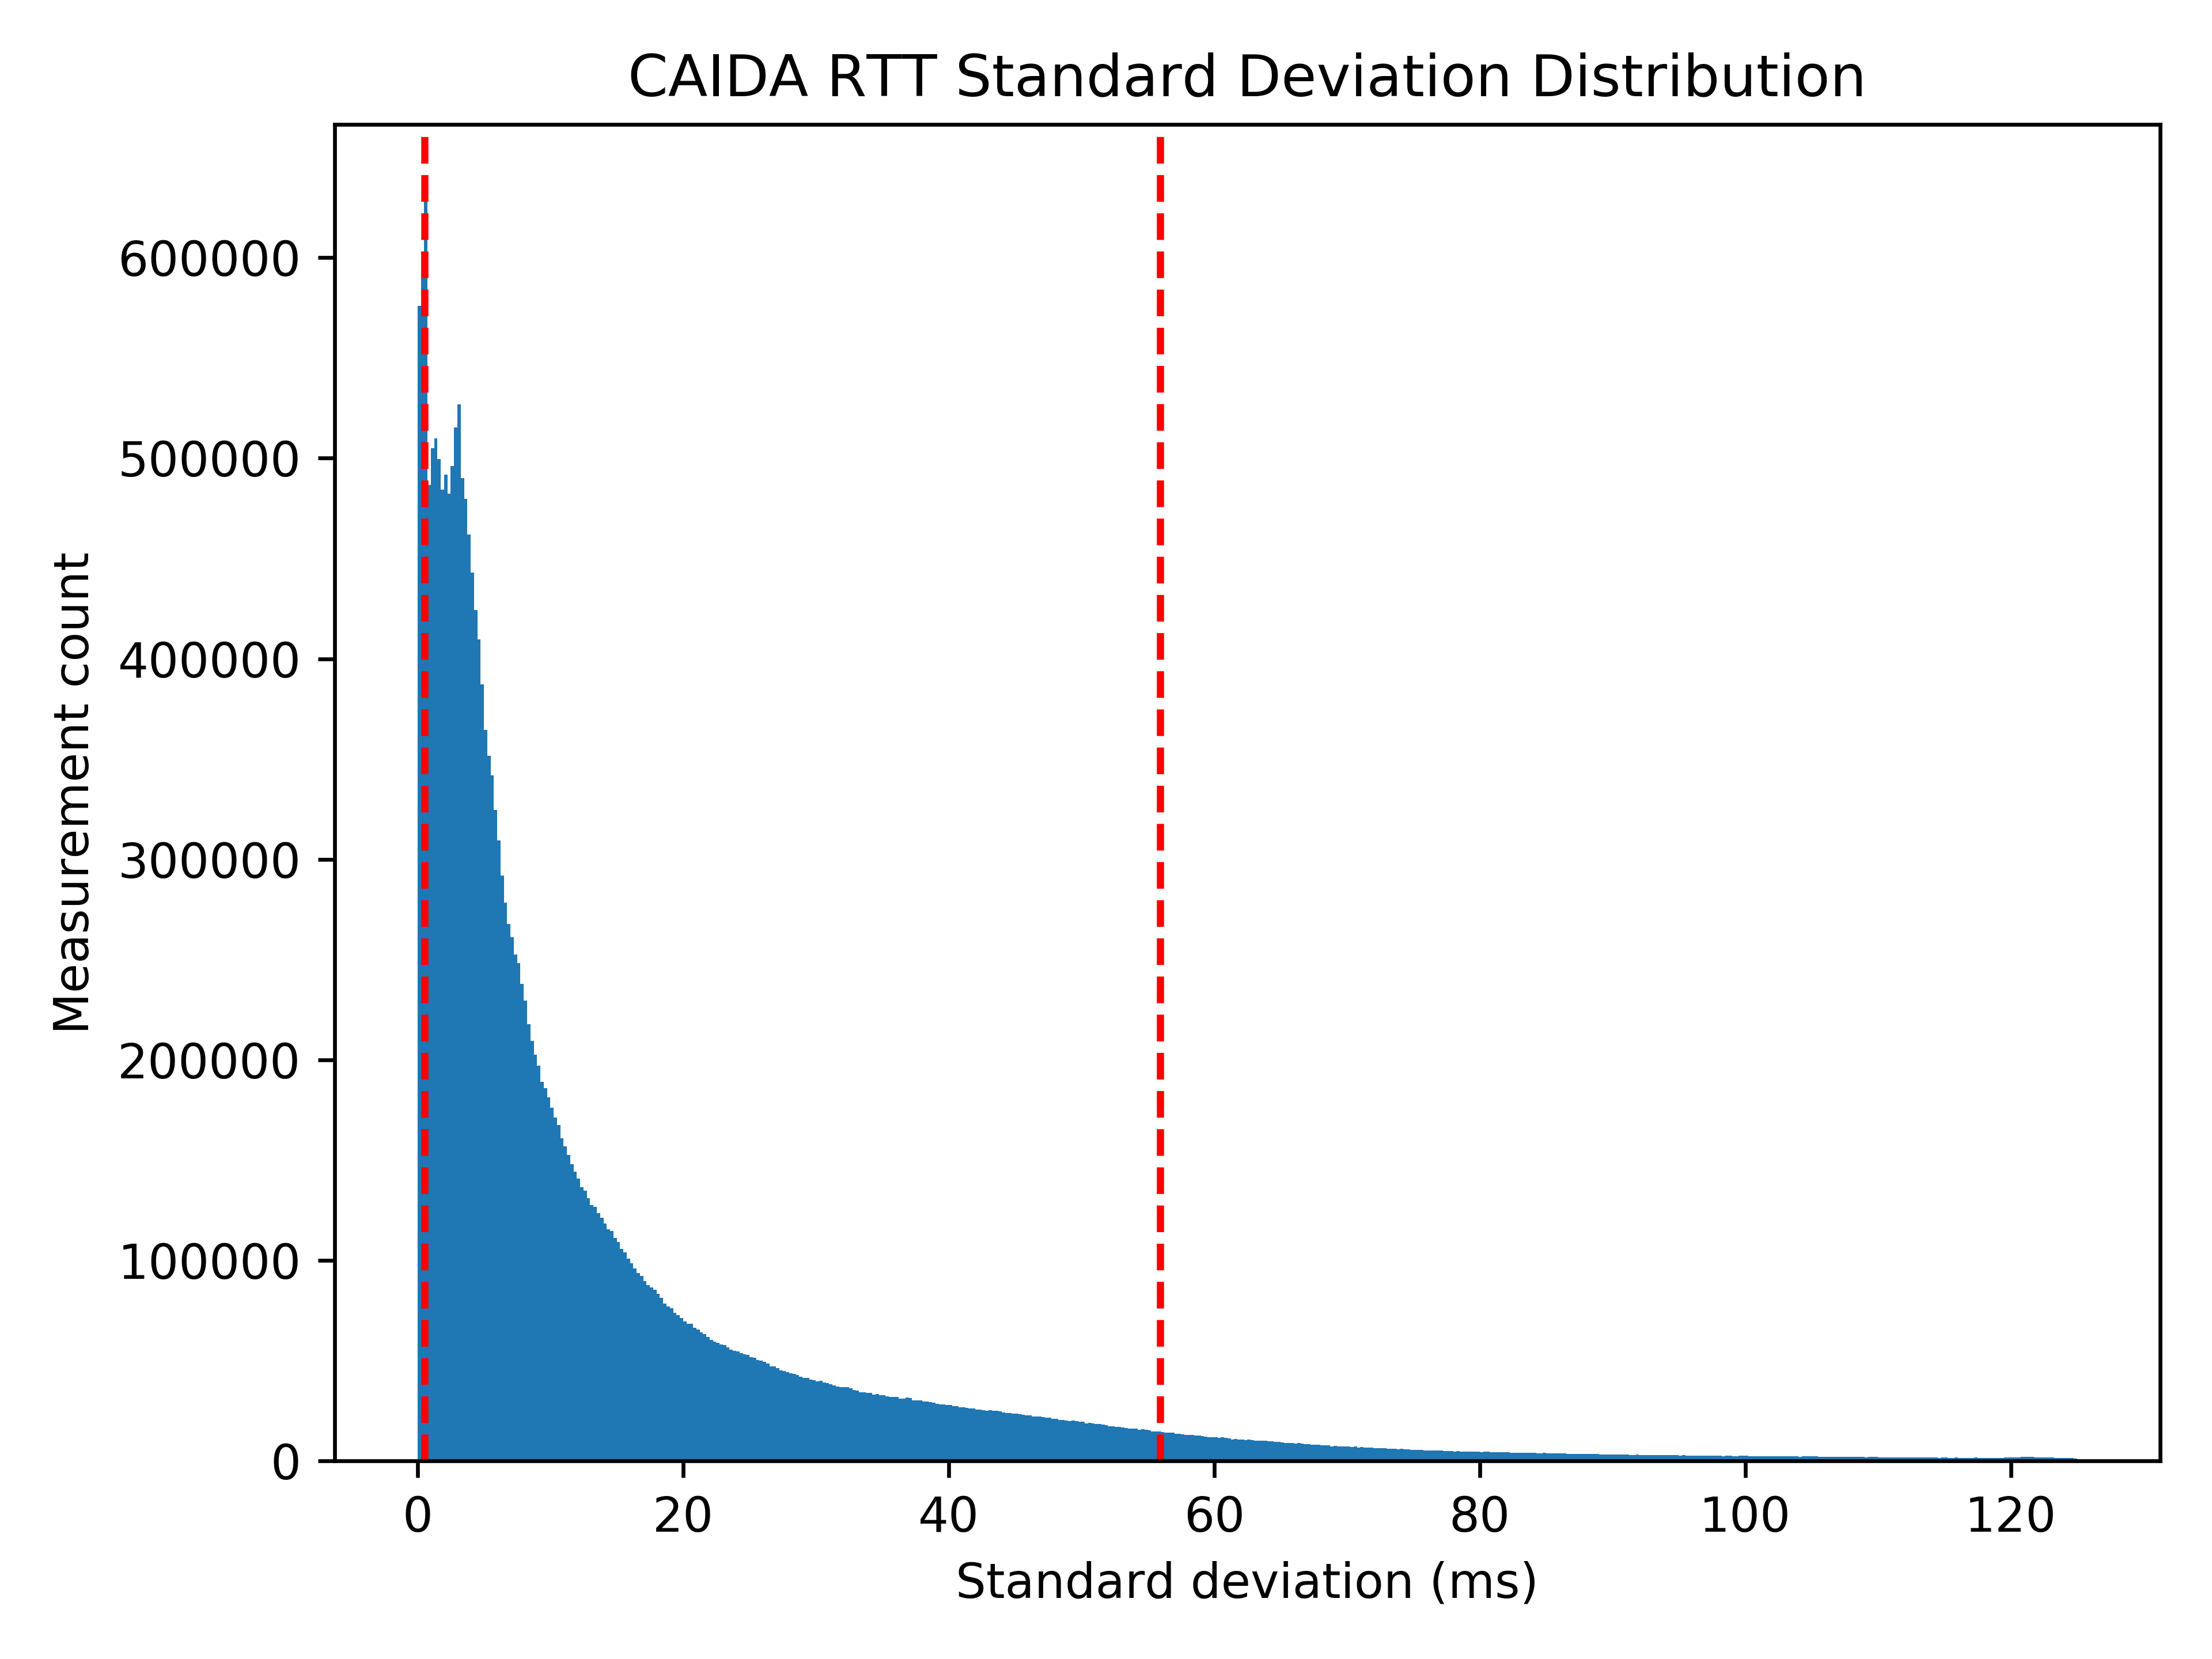
\includegraphics[width=\textwidth]{images/CAIDA_rtt_stdev_dist.png}
    \caption{Distribution of CAIDA RTT standard deviations with 5th and 95th percentiles}
    \label{fig:rtt_stdev_dist}
\end{figure}

Since \acrshort{caida} reports many trials per source-destination pair, a measure of the standard deviations of those measurements is useful to gauge jitter along connections. Figure \ref{fig:rtt_stdev_dist} shows the distribution of standard deviations, which shows a beautifully sloped curve that peaks on the left -- lower standard deviation means lower spread of data, so we can reasonably infer the data is of high quality.

\begin{figure}[H]
    \centering
    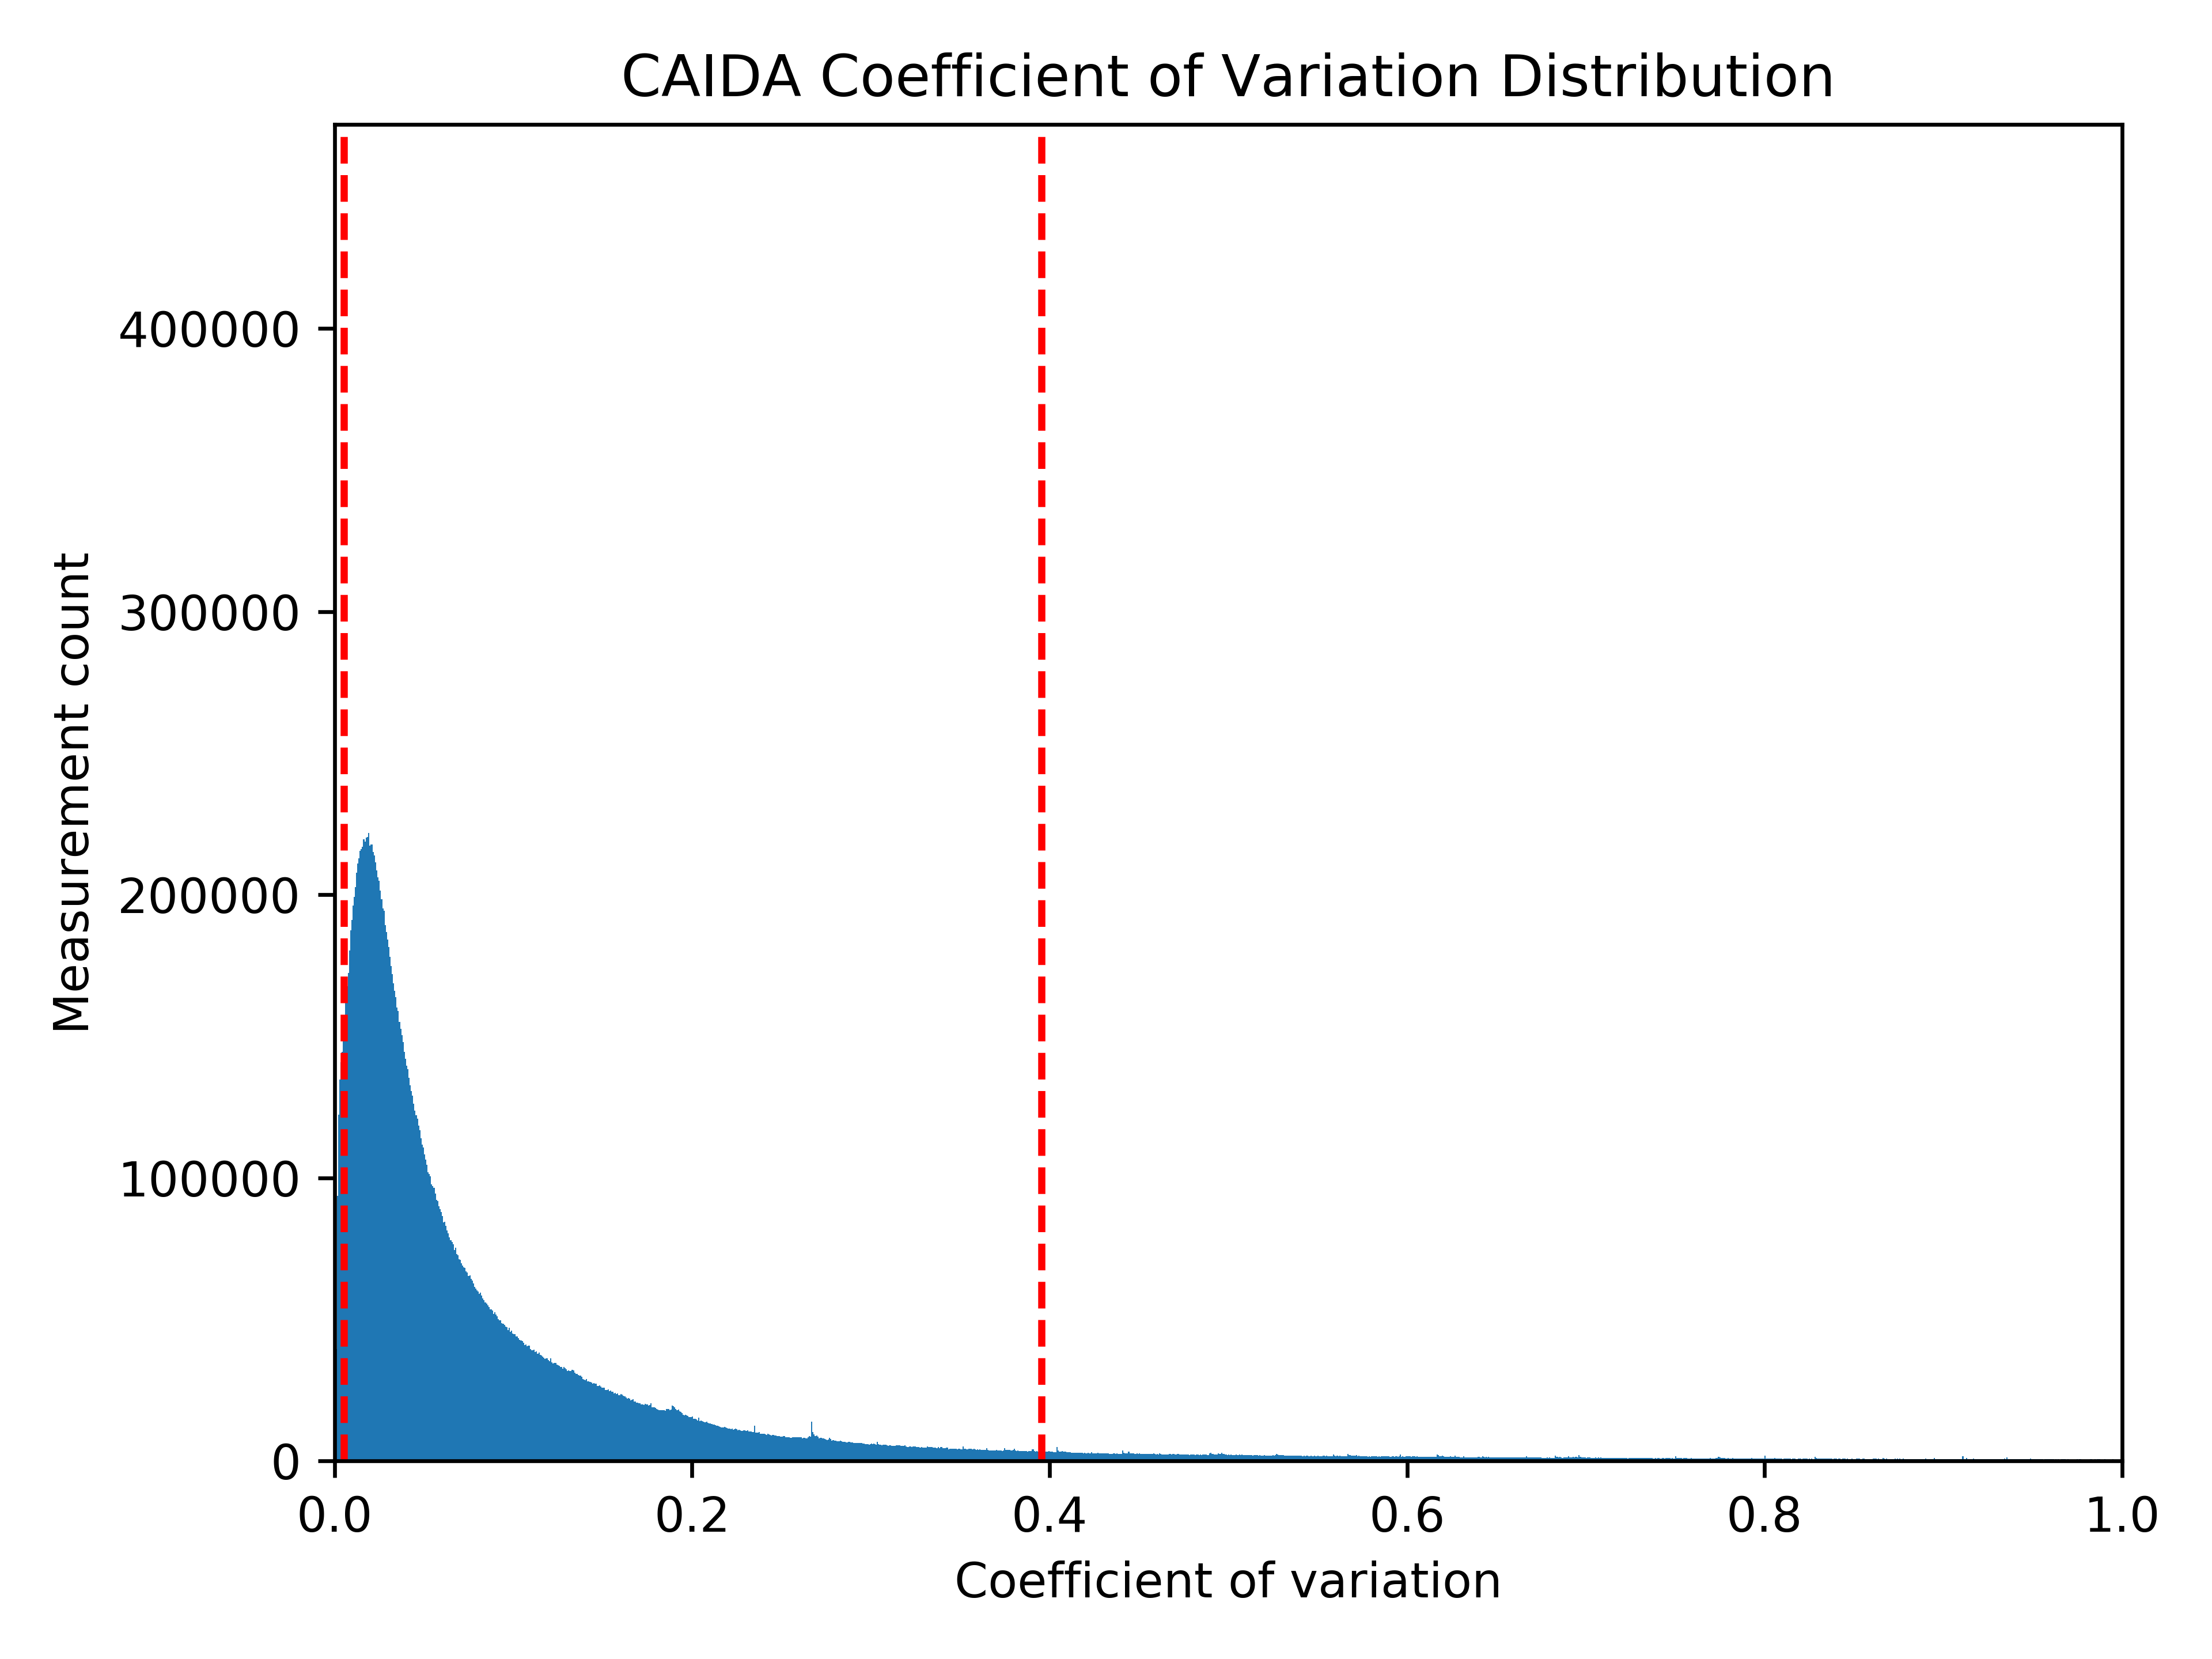
\includegraphics[width=\textwidth]{images/CAIDA_cv_dist.png}
    \caption{Distribution of CAIDA RTT coefficients of variance with 5th and 95th percentiles} 
    \label{fig:rtt_cv_dst}
\end{figure}

To compound on that, figure \ref{fig:rtt_cv_dst} shows a distribution the coefficients of variation for the data set, a dimensionless value that can be interpreted the same regardless of the underlying data. 0-10 is generally considered excellent, 10-20 is good, 20-30 is acceptable, higher above that is questionable. Broadly speaking most of the data is of excellent quality, but this information is definitely useful on setting appropriate limits for filtering.

\subsubsection{Raw RTT}[Chris M.]
Combined, these three data sets give us access to huge amounts of data on the \acrshort{rtt}s between nodes everywhere in the world -- hundreds of millions of machines -- both for end-to-end connections and connections to intermediaries. Since there are many traceroutes for each source-destination pair, we can control for jitter by averaging measurements together and reporting on other common statistics values (range, standard deviation, etc).

Each \acrshort{ip} in the data set can be geo-located to provide us with reasonably accurate locations for every \acrshort{ip} that appears in the dataset. These locations plus the \acrshort{rtt}s can be used to build a heat map that shows what average \acrshort{rtt} looks like from any given location in the US. Filtering can be done to further refine this, e.g. average \acrshort{rtt} to only US servers, only international servers, and so on.

\subsubsection{RTT per distance}[Chris M.]
\acrshort{rtt}s naturally vary with distance, both because the number of nodes in the path tends to increase with path length (increasing routing delays) and because time to get data from point A to point B is governed by the speed of light. The amount an \acrshort{rtt} varies with distance, though, depends on the quality of the infrastructure between connection endpoints, so \acrshort{rtt} divided by distance (in units of ms/km) is a good metric for understanding internet connectivity.

To that that end we've conducted some early data analysis using a subset of the \acrshort{caida} prefix probing dataset, and have generated the following heatmap:

\begin{figure}[H]
    \centering
    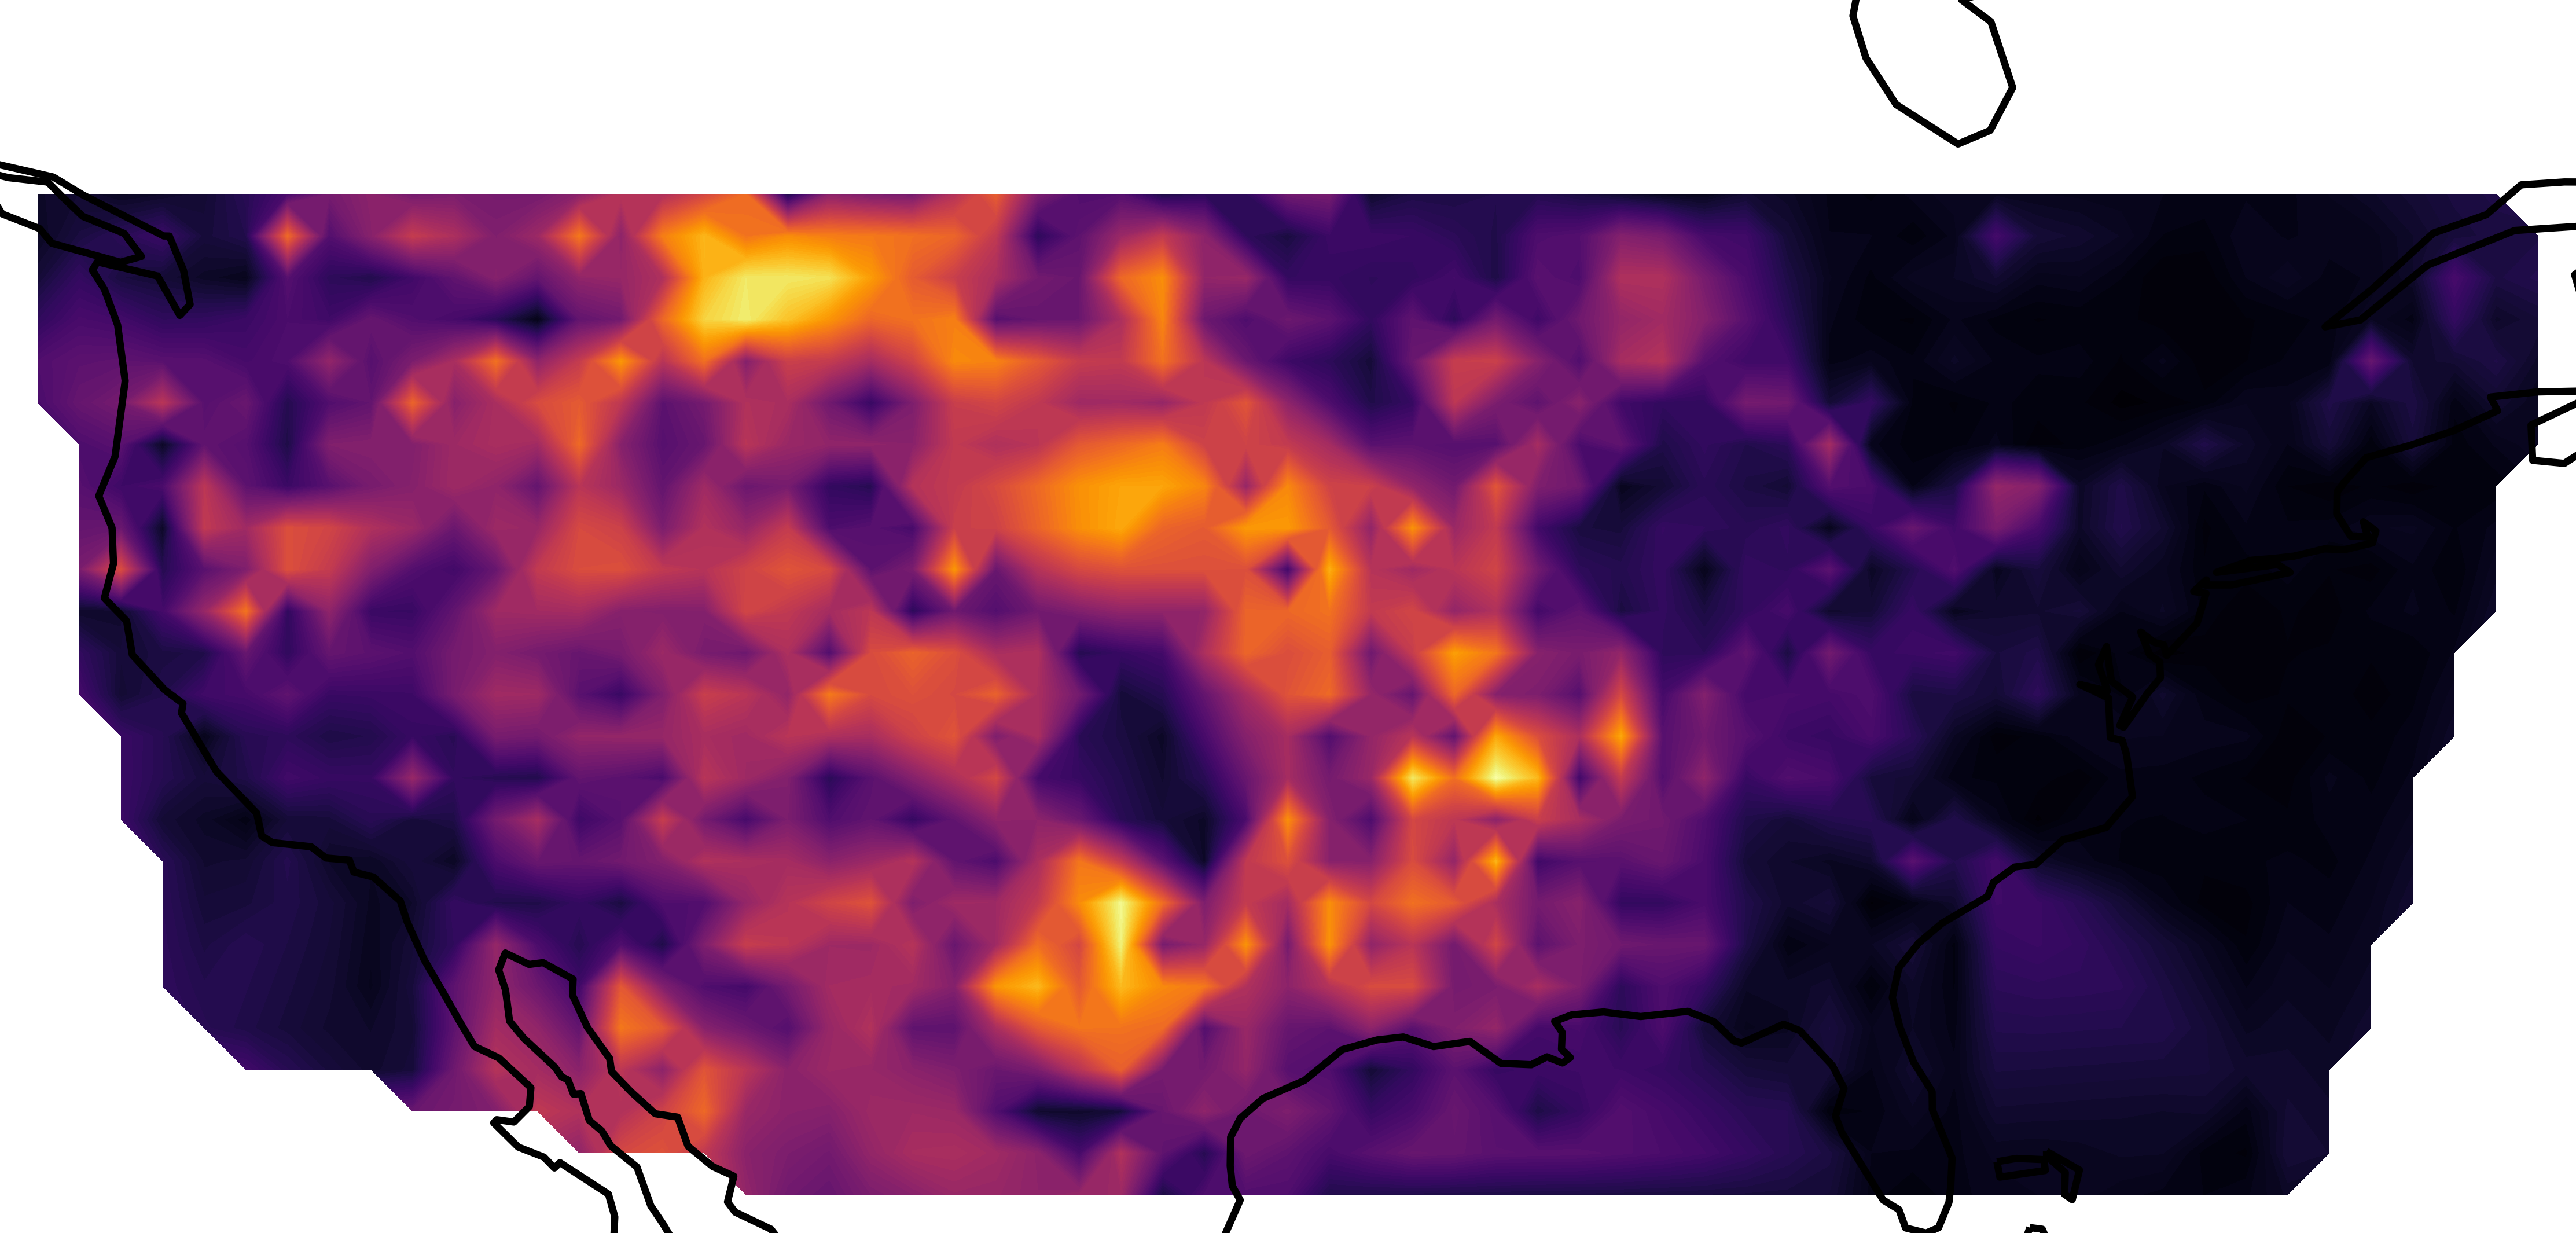
\includegraphics[width=\textwidth]{images/CAIDA_connect_heatmap.png}
    \caption{Heatmap of ms/km values}
    \label{fig:caida_connectivity_heatmap}
\end{figure}

Figure \ref{fig:caida_connectivity_heatmap} shows a heatmap of connectivity across the US where brighter areas correspond to lower internet connectivity. This roughly corresponds to data available from \acrfull{isp}s, which indicate that the Northwest, for instance, generally has much poorer internet access. This map was generated using python matplotlib and some data analysis techniques to reduce the sheer quantity of data from hundreds of millions of data points to only a few thousand (see \S{}\ref{sec:optimization}).

\begin{figure}[H]
    \centering
    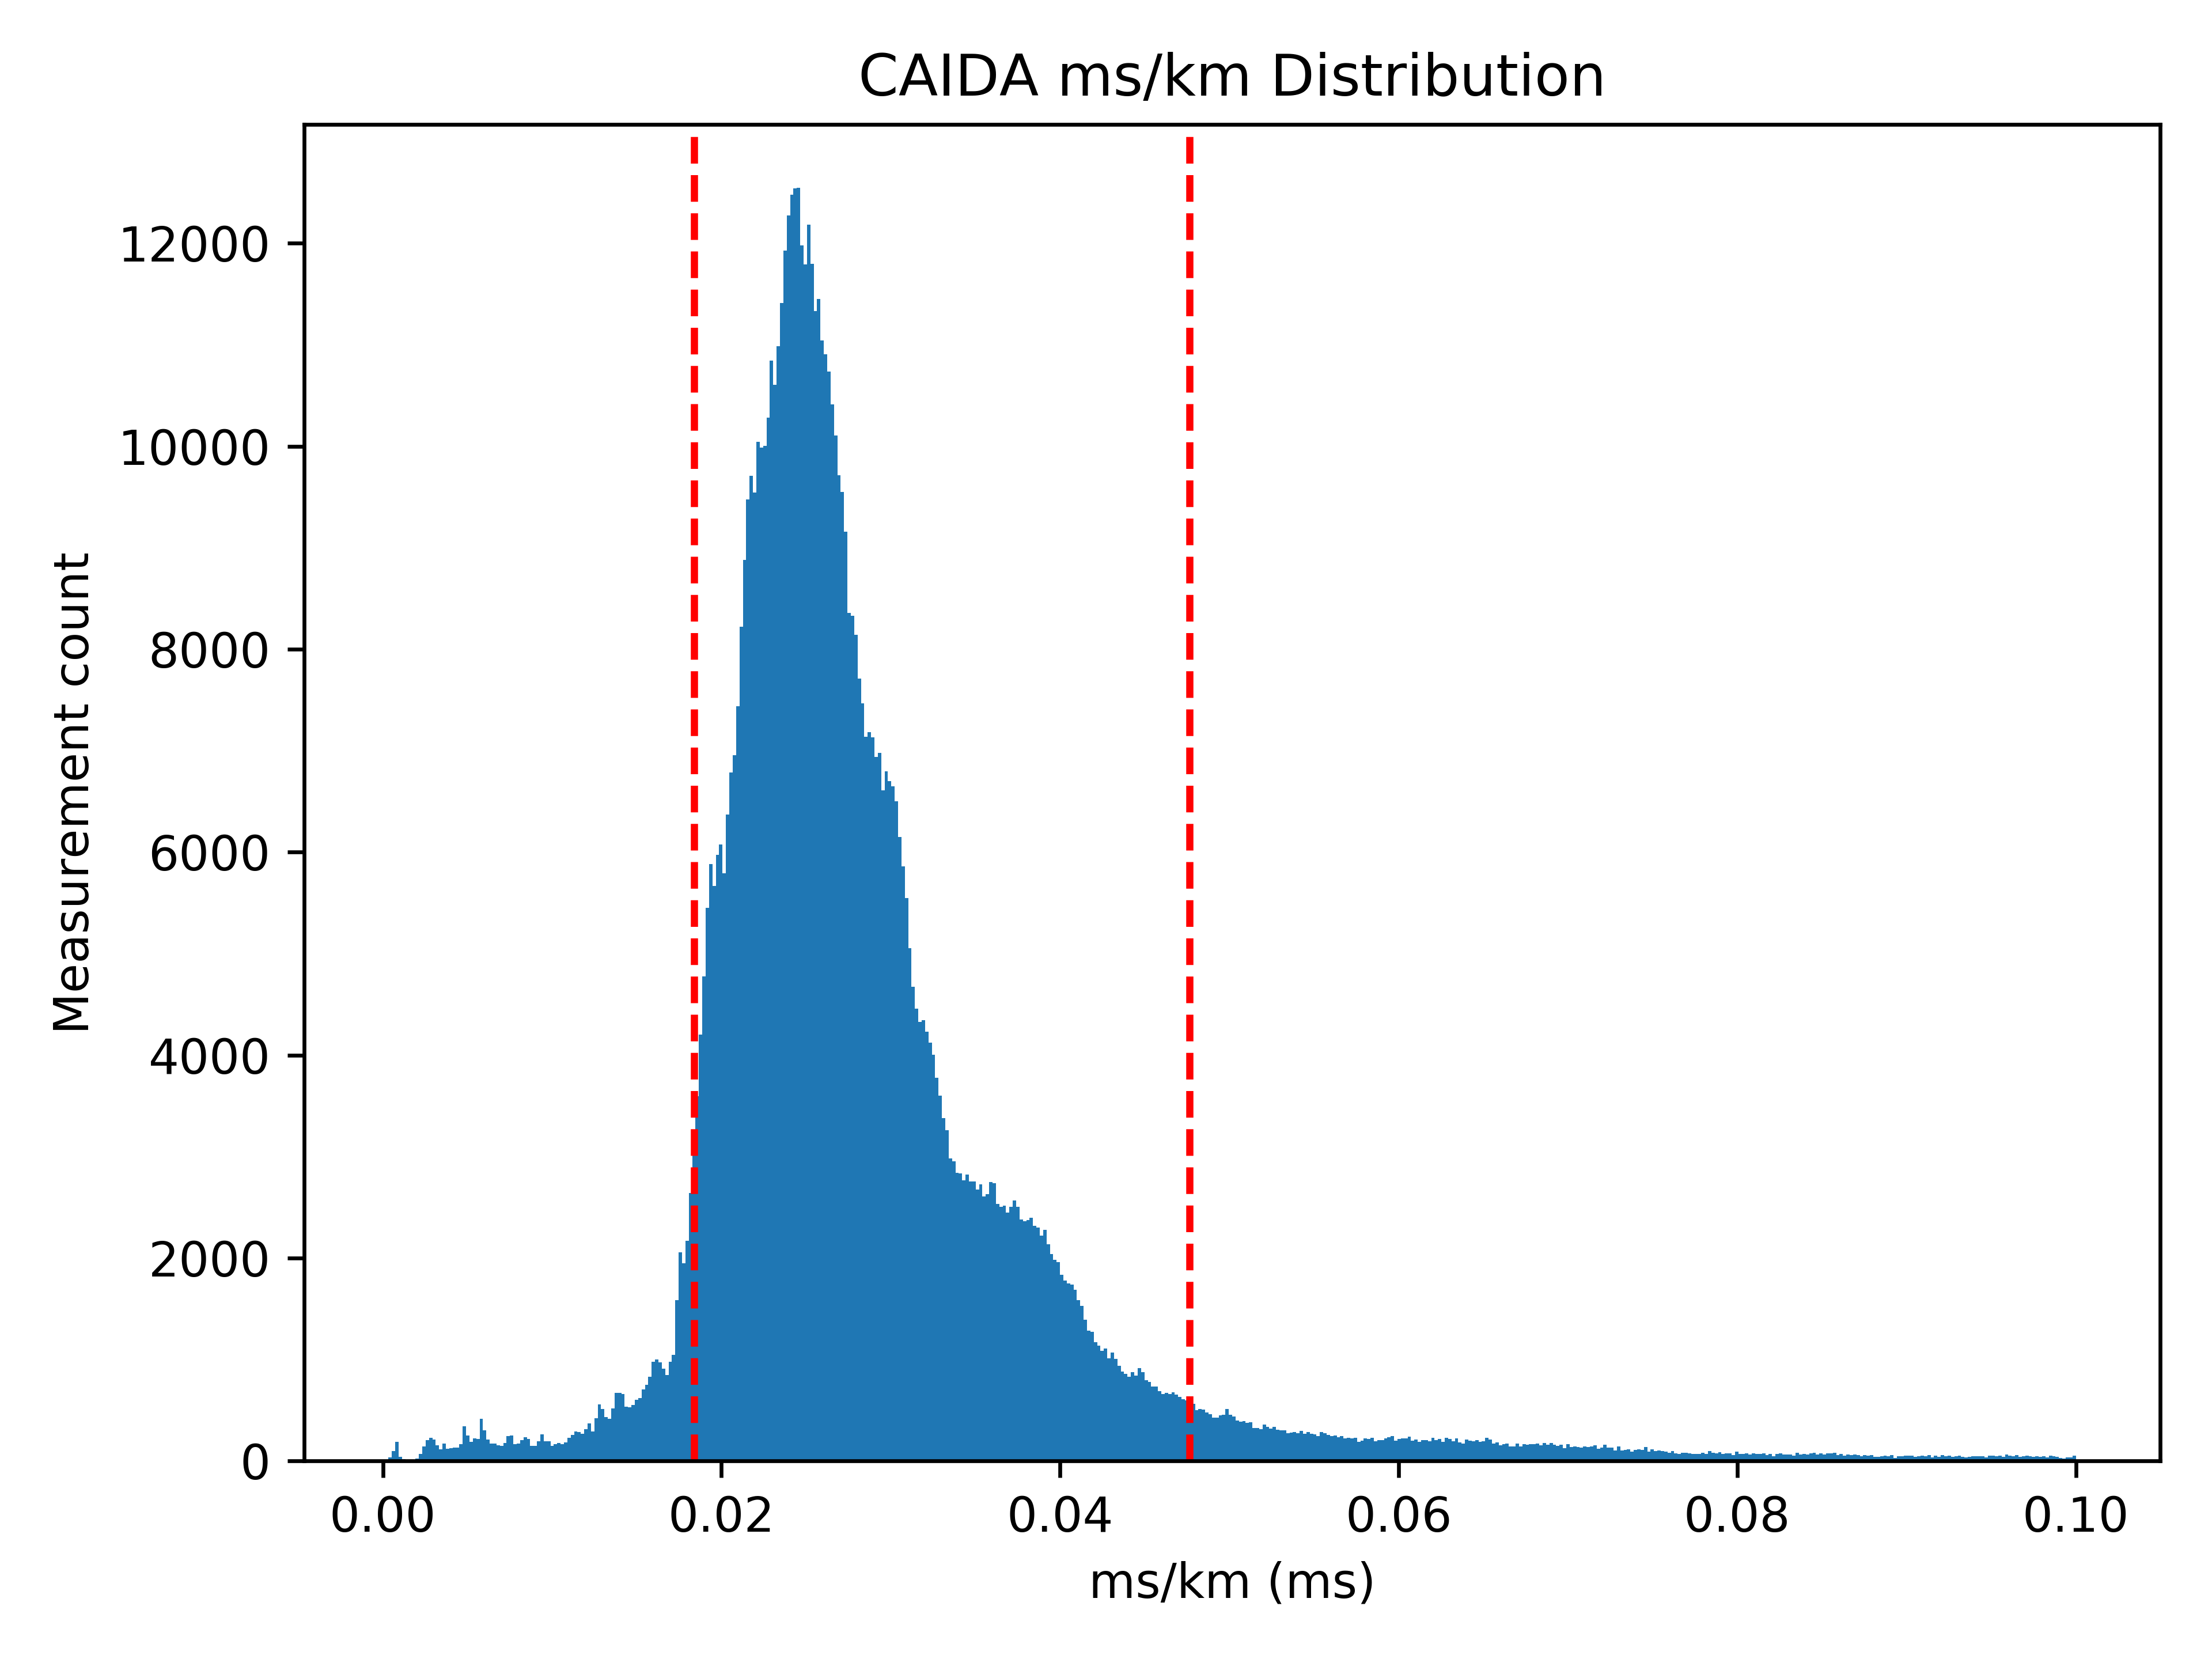
\includegraphics[width=\textwidth]{images/CAIDA_connect_dist.png}
    \caption{Distribution of CAIDA ms/km values with 5th and 95th percentiles}
    \label{fig:caida_connectivity_dist}
\end{figure}

Figure \ref{fig:caida_connectivity_dist} shows is based on the data as figure \ref{fig:caida_connectivity_heatmap}, but shows a distribution instead. This is another fairly narrow peak, but with enough interesting variation and shoulders to hint at underlying patterns and data worth analyzing.

\subsubsection{Backbone analysis}[Chris M.]
\subsubsection{Hops RTT vs. single RTT}[Chris M.]
\label{sec:optimization}\subsubsection{Optimization Techniques \& Database Design}[Chris M.]

To put it mildly, there is a \textit{massive} amount of data to analyze. We estimated about 185 billion datapoints from \acrshort{caida} alone using one method of analysis; even if it's off by an order of magnitude or two, we're still dealing with datapoints in the billions. This amount of raw data is clearly impossible to plot all in one graph, and even if we did, the data would be minimally useful. To that end we've devised a few basic methods for reducing the size of the dataset into something more manageable, without compromising the meaning behind the data. Some of these methods are common statistics and data science techniques, some are not.

\paragraph{Grouping source-destination pairs}

We interpret multiple instances of source to destination pairs as the equivalent of multiple "trials" of an experiment. These values are grouped together and averaged to create a final value. We also calculate the standard deviation and range of the values that formed the average.

\paragraph{Filtering by coefficient of variation}

The coefficient of variation is an ideal quantity for filtering as it doesn't matter what the underlying data set is. We can reduce the data by filtering to source-destination pairs with CVs below 20, for example.

\paragraph{Storing location and IPs separately}

Performing a geo-IP lookup is costly, so caching is preferable. Storing source+destination latitude and longitude alongside each source-destination pair is also costly, with a minimum of 16 extra bytes per row, and when you're dealing with billions of rows, every byte counts. To solve this, locations are cached in a separate table that is joined with the filtered and grouped \acrshort{ip}s instead of with locations for each raw data point.

\paragraph{Quadtree grouping}

The above methods can reduce a \textapprox{}200,000,000 row table to only \textapprox{}800,000 rows, a massive improvement but still too much to chart at once. To solve this we devised a quadtree-based algorithm for grouping nearby points together and averaging them. This is based on the premise that close-together measurement points \textit{should} have roughly similar values. We can't just divide the map into an equally-spaced grid, though, as that would lose a lot of nuance in the data.

The quadtree algorithm works by first assembling a list of all datapoints, finding medians along the horizontal and vertical axes, and splitting into four groups based on those values. The same process is repeated recursively for each child group, with the necessity of a further split determined by exceeding some set level of items, and up to a maximum tree depth that corresponds to the granularity of the resulting map. When put into action and graphed directly, the resulting map looks something like this:

\begin{figure}[H]
    \centering
    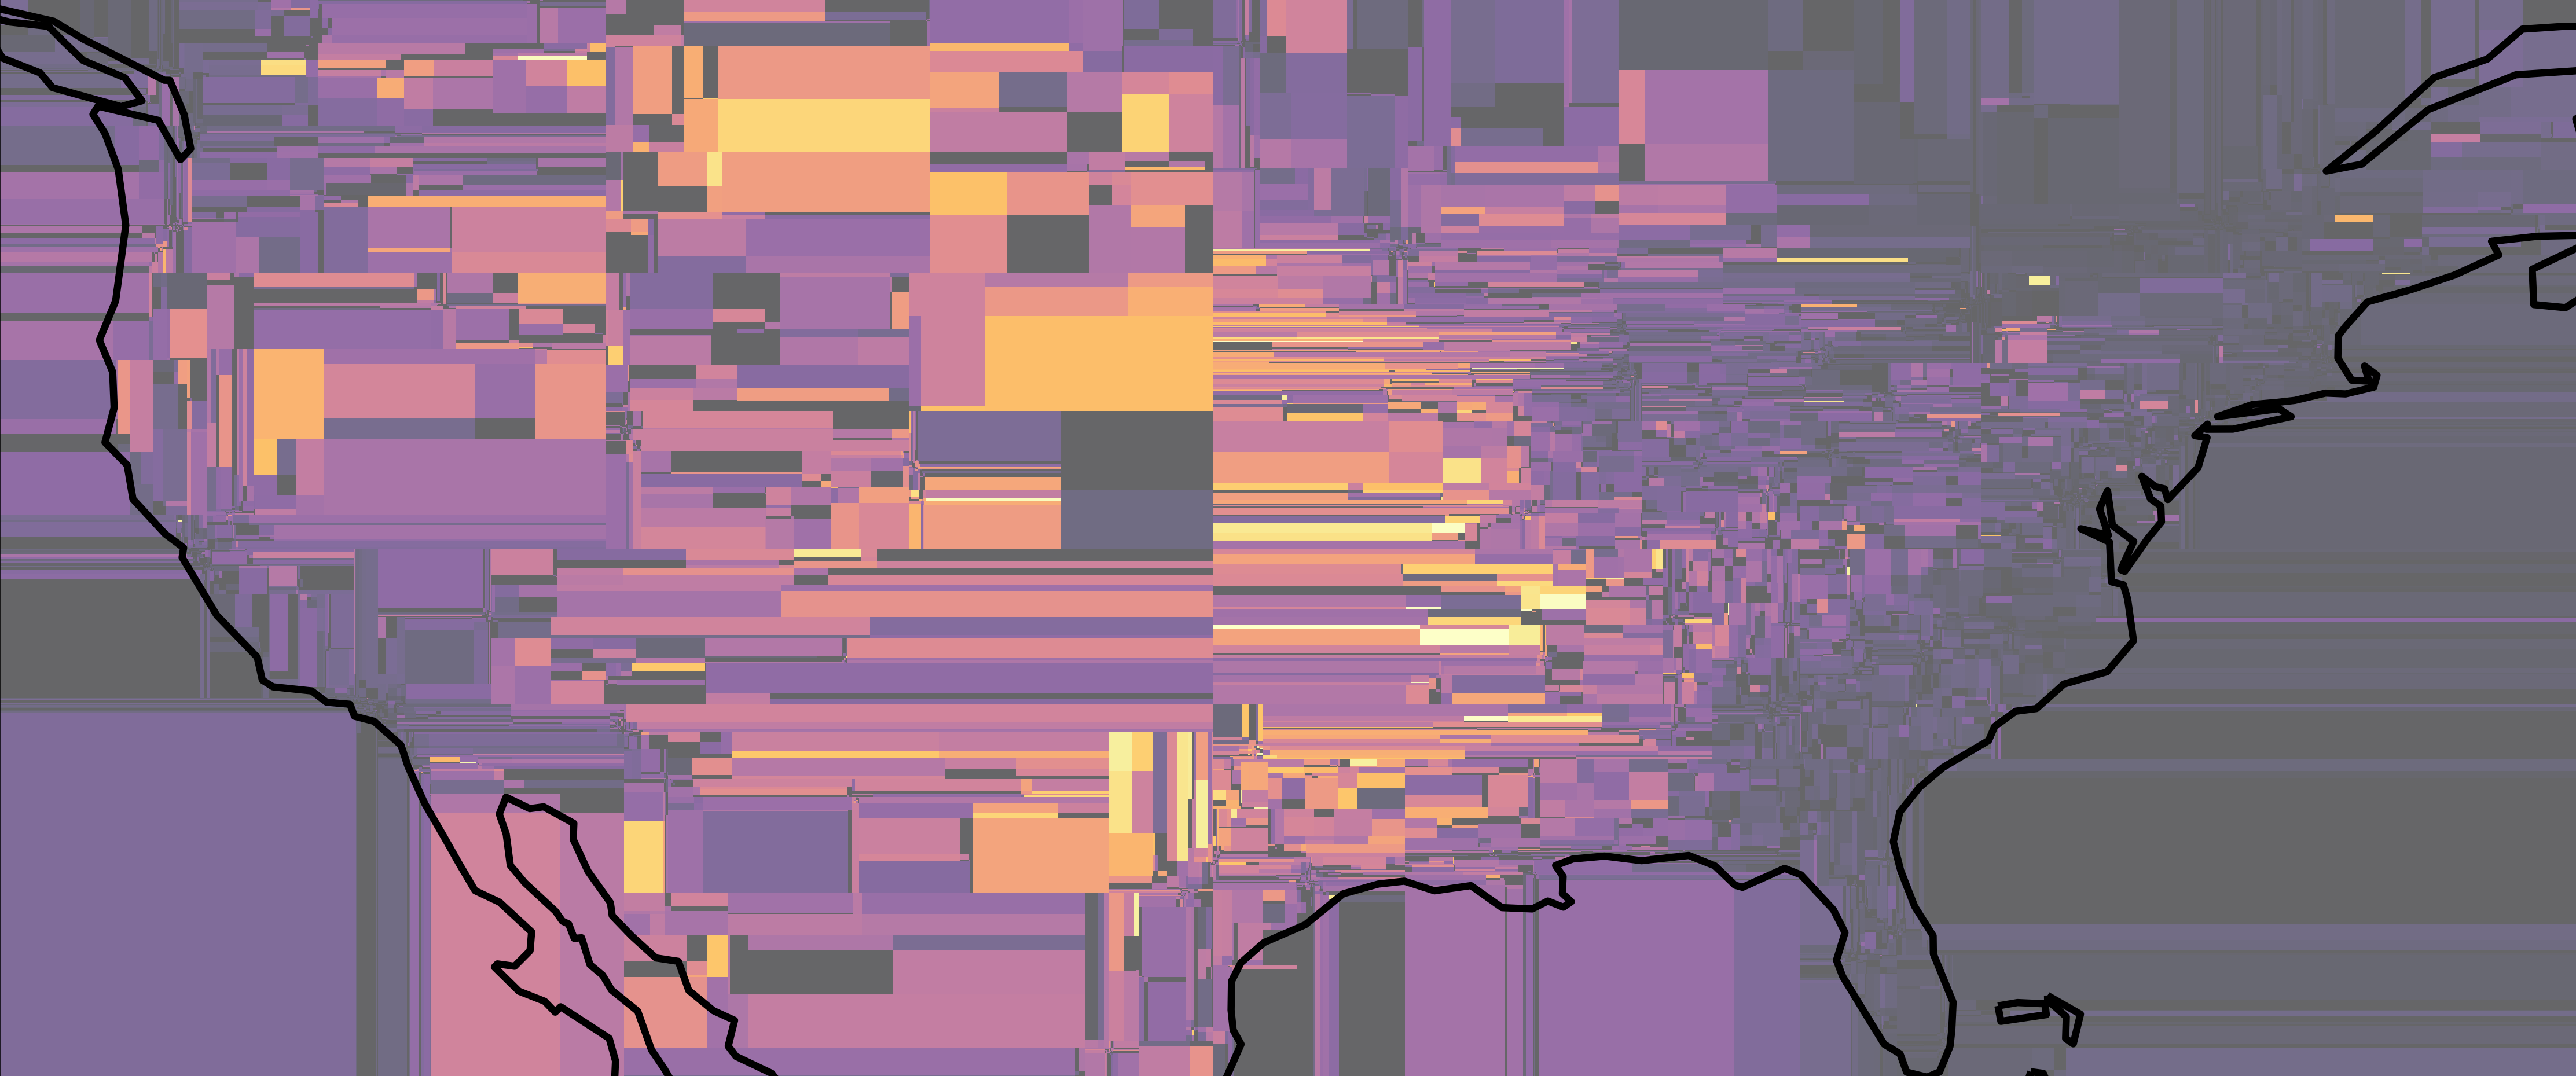
\includegraphics[width=\textwidth]{images/caida_connect_quadplot.png}
    \caption{Ms/km heatmap, quadtree format. Brighter areas indicate higher values.}
    \label{fig:caida_quadplot}
\end{figure}

The smaller the box, the more measurements are in that geographic area. The center of the box is interpreted as a data point and graphed accordingly. Using this technique, the total amount of data points can be reduced from hundreds of thousands to under 1,000, with an average efficiency of about 90\%. This technique was used to generate the heatmap shown in figure \ref{fig:caida_connectivity_heatmap}.

\subsection{ISP Mapping}[David V.]
Using the \acrfull{fcc}'s comprehensive Fixed Broadband Deployment database \cite{FixedMap} we can see what the maximum rated connection speed that is offered in each zip code, as well as the number of \acrshort{isp}s that serve a given area. Another useful data collection method  for this could be asking users on a distributed website what there rated connection is, and that number can be compared to the "Rated" maximum speed. 

\subsubsection{Rated connection speed for given location speed}[David V.]
By mapping the rated connection speed for the given location you can get an idea of the "advertised" connection speeds across the country. This data would be useful for users, especially when compared to the measured speeds from the favicon pings or the \acrshort{caida} data. Comparing these measured data points to the advertised data points could also give people an idea if they are able to get what they are paid for.  

\subsection{Route-trip}[Evan G.]
Using an application on either a mobile device (e.g. smart phone or laptop equipped with mobile broadband and \acrshort{gps}), we could drive across any given area (up to the entire continental United States) and run traceroutes or pings to \acrshort{ip} addresses/domain names for top sites, and record the \acrshort{rtt} along with an exact location. The information collected could be used to measure both cellular infrastructure and 4G connectivity as well as local internet connectivity.

% It's simpler to disable automatic sectioning for the glossaries and references than it is to fix a bug
% in table-of-authorship handling. I'm so, so sorry.
\singlespacing
\let\endsection\section
\renewcommand{\section}[2]{}%

% List of acronyms
\newpage
\endsection{Acronyms}
\setglossarystyle{index} % See https://www.dickimaw-books.com/gallery/glossaries-styles/ for styles
\printglossary[type=\acronymtype]

% Bibliography, automagically managed in IEEE style.
\newpage
\endsection{References}
\bibliographystyle{ieeetr}
\bibliography{references}
\end{document}
